\documentclass{standalone}
\usepackage{tikz}
\usetikzlibrary{patterns, positioning}


\begin{document}
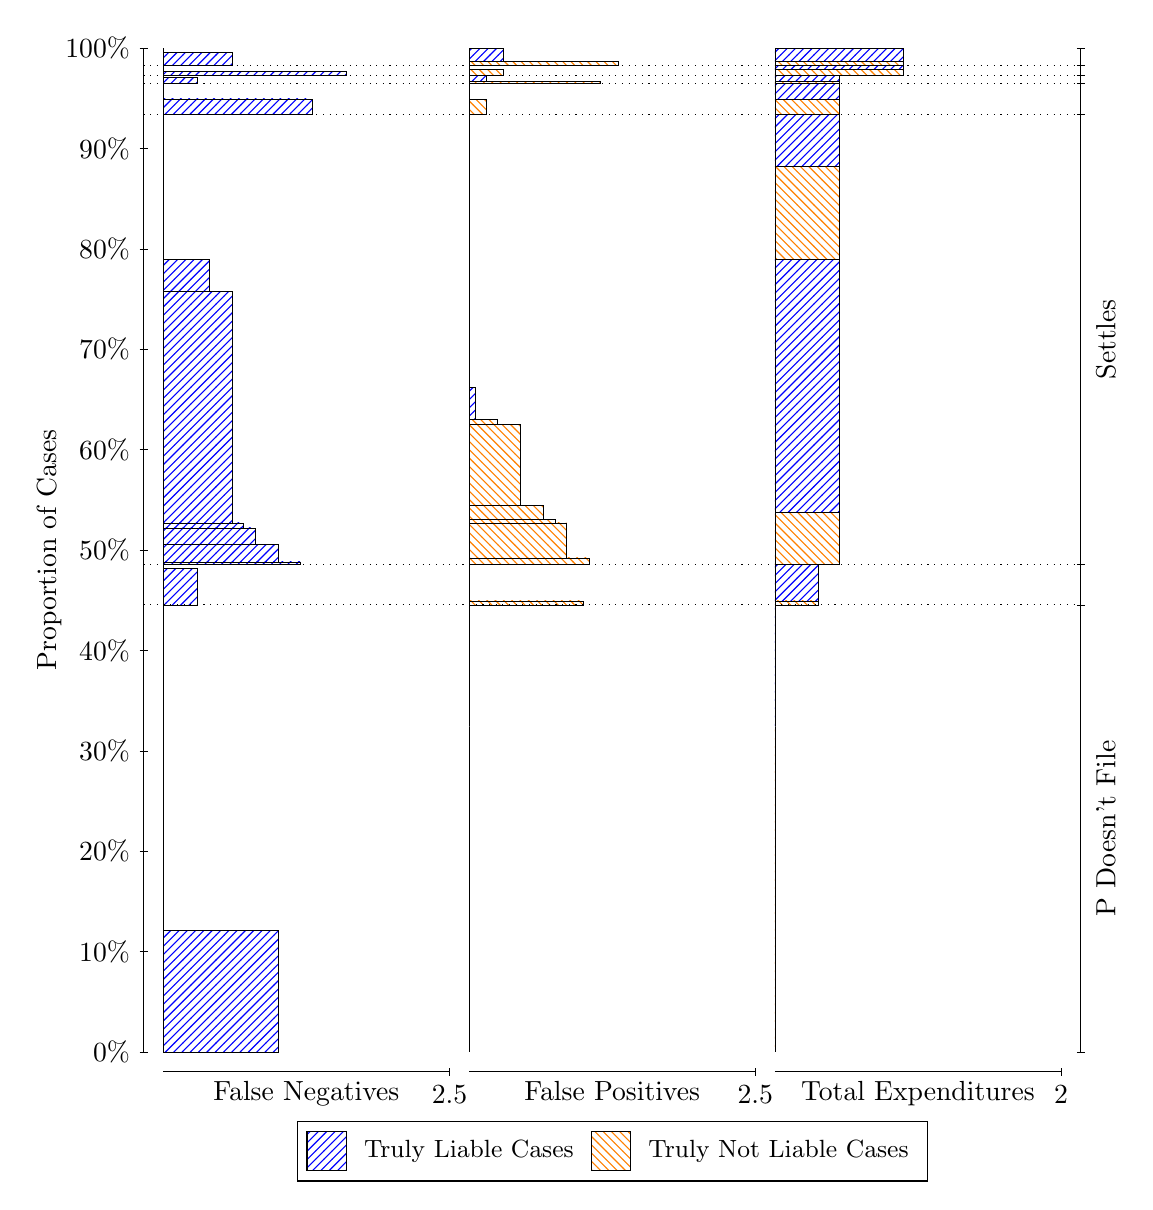
\begin{tikzpicture}
\draw[black, very thin] (1.5,1.75) -- (1.5,14.5);
\node[rotate=90, text=black, anchor=center] at (0.3, 8.125) {Proportion of Cases};
\draw[black, very thin] (1.45,1.75) -- (1.55,1.75);
\node[text=black, anchor=east] at (1.45, 1.75) {0\%};
\draw[black, very thin] (1.45,3.025) -- (1.55,3.025);
\node[text=black, anchor=east] at (1.45, 3.025) {10\%};
\draw[black, very thin] (1.45,4.3) -- (1.55,4.3);
\node[text=black, anchor=east] at (1.45, 4.3) {20\%};
\draw[black, very thin] (1.45,5.575) -- (1.55,5.575);
\node[text=black, anchor=east] at (1.45, 5.575) {30\%};
\draw[black, very thin] (1.45,6.85) -- (1.55,6.85);
\node[text=black, anchor=east] at (1.45, 6.85) {40\%};
\draw[black, very thin] (1.45,8.125) -- (1.55,8.125);
\node[text=black, anchor=east] at (1.45, 8.125) {50\%};
\draw[black, very thin] (1.45,9.4) -- (1.55,9.4);
\node[text=black, anchor=east] at (1.45, 9.4) {60\%};
\draw[black, very thin] (1.45,10.675) -- (1.55,10.675);
\node[text=black, anchor=east] at (1.45, 10.675) {70\%};
\draw[black, very thin] (1.45,11.95) -- (1.55,11.95);
\node[text=black, anchor=east] at (1.45, 11.95) {80\%};
\draw[black, very thin] (1.45,13.225) -- (1.55,13.225);
\node[text=black, anchor=east] at (1.45, 13.225) {90\%};
\draw[black, very thin] (1.45,14.5) -- (1.55,14.5);
\node[text=black, anchor=east] at (1.45, 14.5) {100\%};

\draw[black, very thin] (13.4,1.75) -- (13.4,14.5);
\draw[black, very thin] (13.35,1.75) -- (13.45,1.75);
\node[anchor=west] at (13.35, 1.75) {};
\draw[black, very thin] (13.35,7.4277) -- (13.45,7.4277);
\node[anchor=west] at (13.35, 7.4277) {};
\draw[black, very thin] (13.35,7.9425) -- (13.45,7.9425);
\node[anchor=west] at (13.35, 7.9425) {};
\draw[black, very thin] (13.35,13.659) -- (13.45,13.659);
\node[anchor=west] at (13.35, 13.659) {};
\draw[black, very thin] (13.35,14.049) -- (13.45,14.049);
\node[anchor=west] at (13.35, 14.049) {};
\draw[black, very thin] (13.35,14.154) -- (13.45,14.154);
\node[anchor=west] at (13.35, 14.154) {};
\draw[black, very thin] (13.35,14.28) -- (13.45,14.28);
\node[anchor=west] at (13.35, 14.28) {};
\draw[black, very thin] (13.35,14.5) -- (13.45,14.5);
\node[anchor=west] at (13.35, 14.5) {};

\draw[black, very thin, pattern color=blue, pattern=north east lines] (1.75,1.75) rectangle (3.2033,3.2933);
\draw[black, very thin, pattern color=orange, pattern=north west lines] (1.75,3.2933) rectangle (1.75,7.4277);
\draw[black, very thin, pattern color=blue, pattern=north east lines] (1.75,7.4277) rectangle (2.186,7.8913);
\draw[black, very thin, pattern color=orange, pattern=north west lines] (1.75,7.8913) rectangle (1.75,7.9425);
\draw[black, very thin, pattern color=blue, pattern=north east lines] (1.75,7.9425) rectangle (3.494,7.9732);
\draw[black, very thin, pattern color=blue, pattern=north east lines] (1.75,7.9732) rectangle (3.2033,8.1972);
\draw[black, very thin, pattern color=blue, pattern=north east lines] (1.75,8.1972) rectangle (2.9127,8.4047);
\draw[black, very thin, pattern color=blue, pattern=north east lines] (1.75,8.4047) rectangle (2.7673,8.4685);
\draw[black, very thin, pattern color=blue, pattern=north east lines] (1.75,8.4685) rectangle (2.622,11.412);
\draw[black, very thin, pattern color=blue, pattern=north east lines] (1.75,11.412) rectangle (2.3313,11.816);
\draw[black, very thin, pattern color=orange, pattern=north west lines] (1.75,11.816) rectangle (1.75,13.659);
\draw[black, very thin, pattern color=blue, pattern=north east lines] (1.75,13.659) rectangle (3.6393,13.855);
\draw[black, very thin, pattern color=orange, pattern=north west lines] (1.75,13.855) rectangle (1.75,14.049);
\draw[black, very thin, pattern color=blue, pattern=north east lines] (1.75,14.049) rectangle (2.186,14.127);
\draw[black, very thin, pattern color=orange, pattern=north west lines] (1.75,14.127) rectangle (1.75,14.154);
\draw[black, very thin, pattern color=blue, pattern=north east lines] (1.75,14.154) rectangle (4.0753,14.208);
\draw[black, very thin, pattern color=orange, pattern=north west lines] (1.75,14.208) rectangle (1.75,14.28);
\draw[black, very thin, pattern color=blue, pattern=north east lines] (1.75,14.28) rectangle (2.622,14.445);
\draw[black, very thin, pattern color=orange, pattern=north west lines] (1.75,14.445) rectangle (1.75,14.5);
\draw[black, very thin, pattern color=orange, pattern=north west lines] (5.6333,1.75) rectangle (5.6333,5.8844);
\draw[black, very thin, pattern color=blue, pattern=north east lines] (5.6333,5.8844) rectangle (5.6333,7.4277);
\draw[black, very thin, pattern color=orange, pattern=north west lines] (5.6333,7.4277) rectangle (7.0867,7.4789);
\draw[black, very thin, pattern color=blue, pattern=north east lines] (5.6333,7.4789) rectangle (5.6333,7.9425);
\draw[black, very thin, pattern color=orange, pattern=north west lines] (5.6333,7.9425) rectangle (7.1593,8.0248);
\draw[black, very thin, pattern color=orange, pattern=north west lines] (5.6333,8.0248) rectangle (6.8687,8.4692);
\draw[black, very thin, pattern color=orange, pattern=north west lines] (5.6333,8.4692) rectangle (6.7233,8.5121);
\draw[black, very thin, pattern color=orange, pattern=north west lines] (5.6333,8.5121) rectangle (6.578,8.6876);
\draw[black, very thin, pattern color=orange, pattern=north west lines] (5.6333,8.6876) rectangle (6.2873,9.7157);
\draw[black, very thin, pattern color=orange, pattern=north west lines] (5.6333,9.7157) rectangle (5.9967,9.7851);
\draw[black, very thin, pattern color=blue, pattern=north east lines] (5.6333,9.7851) rectangle (5.706,10.19);
\draw[black, very thin, pattern color=blue, pattern=north east lines] (5.6333,10.19) rectangle (5.6333,13.659);
\draw[black, very thin, pattern color=orange, pattern=north west lines] (5.6333,13.659) rectangle (5.8513,13.852);
\draw[black, very thin, pattern color=blue, pattern=north east lines] (5.6333,13.852) rectangle (5.6333,14.049);
\draw[black, very thin, pattern color=orange, pattern=north west lines] (5.6333,14.049) rectangle (7.3047,14.076);
\draw[black, very thin, pattern color=blue, pattern=north east lines] (5.6333,14.076) rectangle (5.8513,14.154);
\draw[black, very thin, pattern color=orange, pattern=north west lines] (5.6333,14.154) rectangle (6.0693,14.226);
\draw[black, very thin, pattern color=blue, pattern=north east lines] (5.6333,14.226) rectangle (5.6333,14.28);
\draw[black, very thin, pattern color=orange, pattern=north west lines] (5.6333,14.28) rectangle (7.5227,14.335);
\draw[black, very thin, pattern color=blue, pattern=north east lines] (5.6333,14.335) rectangle (6.0693,14.5);
\draw[black, very thin, pattern color=orange, pattern=north west lines] (9.5167,1.75) rectangle (9.5167,5.8844);
\draw[black, very thin, pattern color=blue, pattern=north east lines] (9.5167,5.8844) rectangle (9.5167,7.4277);
\draw[black, very thin, pattern color=orange, pattern=north west lines] (9.5167,7.4277) rectangle (10.062,7.4789);
\draw[black, very thin, pattern color=blue, pattern=north east lines] (9.5167,7.4789) rectangle (10.062,7.9425);
\draw[black, very thin, pattern color=orange, pattern=north west lines] (9.5167,7.9425) rectangle (10.334,8.6053);
\draw[black, very thin, pattern color=blue, pattern=north east lines] (9.5167,8.6053) rectangle (10.334,11.82);
\draw[black, very thin, pattern color=orange, pattern=north west lines] (9.5167,11.82) rectangle (10.334,13);
\draw[black, very thin, pattern color=blue, pattern=north east lines] (9.5167,13) rectangle (10.334,13.659);
\draw[black, very thin, pattern color=orange, pattern=north west lines] (9.5167,13.659) rectangle (10.334,13.852);
\draw[black, very thin, pattern color=blue, pattern=north east lines] (9.5167,13.852) rectangle (10.334,14.049);
\draw[black, very thin, pattern color=orange, pattern=north west lines] (9.5167,14.049) rectangle (10.334,14.076);
\draw[black, very thin, pattern color=blue, pattern=north east lines] (9.5167,14.076) rectangle (10.334,14.154);
\draw[black, very thin, pattern color=orange, pattern=north west lines] (9.5167,14.154) rectangle (11.152,14.226);
\draw[black, very thin, pattern color=blue, pattern=north east lines] (9.5167,14.226) rectangle (11.152,14.28);
\draw[black, very thin, pattern color=orange, pattern=north west lines] (9.5167,14.28) rectangle (11.152,14.335);
\draw[black, very thin, pattern color=blue, pattern=north east lines] (9.5167,14.335) rectangle (11.152,14.5);
\draw[black, dotted] (1.5,7.4277) -- (13.4,7.4277);
\draw[black, dotted] (1.5,7.9425) -- (13.4,7.9425);
\draw[black, dotted] (1.5,13.659) -- (13.4,13.659);
\draw[black, dotted] (1.5,14.049) -- (13.4,14.049);
\draw[black, dotted] (1.5,14.154) -- (13.4,14.154);
\draw[black, dotted] (1.5,14.28) -- (13.4,14.28);
\draw[black, very thin] (1.75,1.5) -- (5.3833,1.5);
\node[text=black, anchor=north] at (3.5667, 1.5) {False Negatives};
\draw[black, very thin] (5.3833,1.45) -- (5.3833,1.55);
\node[text=black, anchor=north] at (5.3833, 1.45) {2.5};

\draw[black, very thin] (5.6333,1.5) -- (9.2667,1.5);
\node[text=black, anchor=north] at (7.45, 1.5) {False Positives};
\draw[black, very thin] (9.2667,1.45) -- (9.2667,1.55);
\node[text=black, anchor=north] at (9.2667, 1.45) {2.5};

\draw[black, very thin] (9.5167,1.5) -- (13.15,1.5);
\node[text=black, anchor=north] at (11.333, 1.5) {Total Expenditures};
\draw[black, very thin] (13.15,1.45) -- (13.15,1.55);
\node[text=black, anchor=north] at (13.15, 1.45) {2};

\node[text=black, centered, rotate=90] at (13.72, 4.5888) {P Doesn't File};

\node[text=black, centered, rotate=90] at (13.72, 10.801) {Settles};





\draw (7.449999999999999,1.5) node[draw=none] (baseCoordinate) {};
\begin{scope}[align=center]
        \matrix[scale=0.5, draw=black, below=0.5cm of baseCoordinate, nodes={draw}, column sep=0.1cm]{
            \node[rectangle, draw, minimum width=0.5cm, minimum height=0.5cm, pattern color=blue, pattern=north east lines] {}; &
            \node[draw=none, font=\small, text=black] (B) {Truly Liable Cases}; &
            \node[rectangle, draw, minimum width=0.5cm, minimum height=0.5cm, pattern color=orange, pattern=north west lines] {}; &
            \node[draw=none, font=\small, text=black] (B) {Truly Not Liable Cases}; \\
            };
\end{scope}

\end{tikzpicture}
\end{document}